%TEX root = ../dissertation.tex

\chapter{Implementation}
\label{chapter:implementation}

For our Pulsarcast implementation we decided to take advantage of the
\emph{libp2p} ecosystem as it solves a lot of the underlying issues of building
a peer to peer system, not specific to our pubsub scenario. This includes
dealing with connection multiplexing, NAT traversal, discovery mechanisms, etc.
All of which libp2p, a community focused project with implementations in
multiple languages already solves. We can also take advantage of the utility
modules it has and the advantage of having an already working implementation of
the Kadmelia DHT. Our focus is then to build a module, implementing the
Pulsarcast specification, that clients and apps can take advantage of. Section
\ref{pulsarcast-javascript-module} provides a detailed description of it.

Besides our module, we also needed to find a suitable way to test our system as
whole. Given our specific needs, we opted to build a custom testbed, detailed
in section \ref{testbed} and the basis of the evaluation detailed in chapter
\ref{chapter:evaluation}. 

\section{Pulscarcast Javascript module}\label{pulsarcast-javascript-module}

We chose to implement our Pulsarcast module in Javascript. As it was covered in
our related work, Javascript is ubiquitous, running in browsers, servers and
many different kinds of devices and architectures. Through it, we are able to
run our Pulscarcast nodes in a multitude of systems and most importantly,
direct its usage for the World Wide Web. Plus, libp2p has a Javascript
implementation focused on cross compatibility between server and browser. This
is not to say that in the future we will not have other implementations in
different languages, that is in fact one of the reasons for the clear
separation between the Pulcarcast specification and its actual implementation.
However, we had to choose, and in our view Javascript is the clear winner.

TODO next

\begin{figure}[hb!]
  \centering
  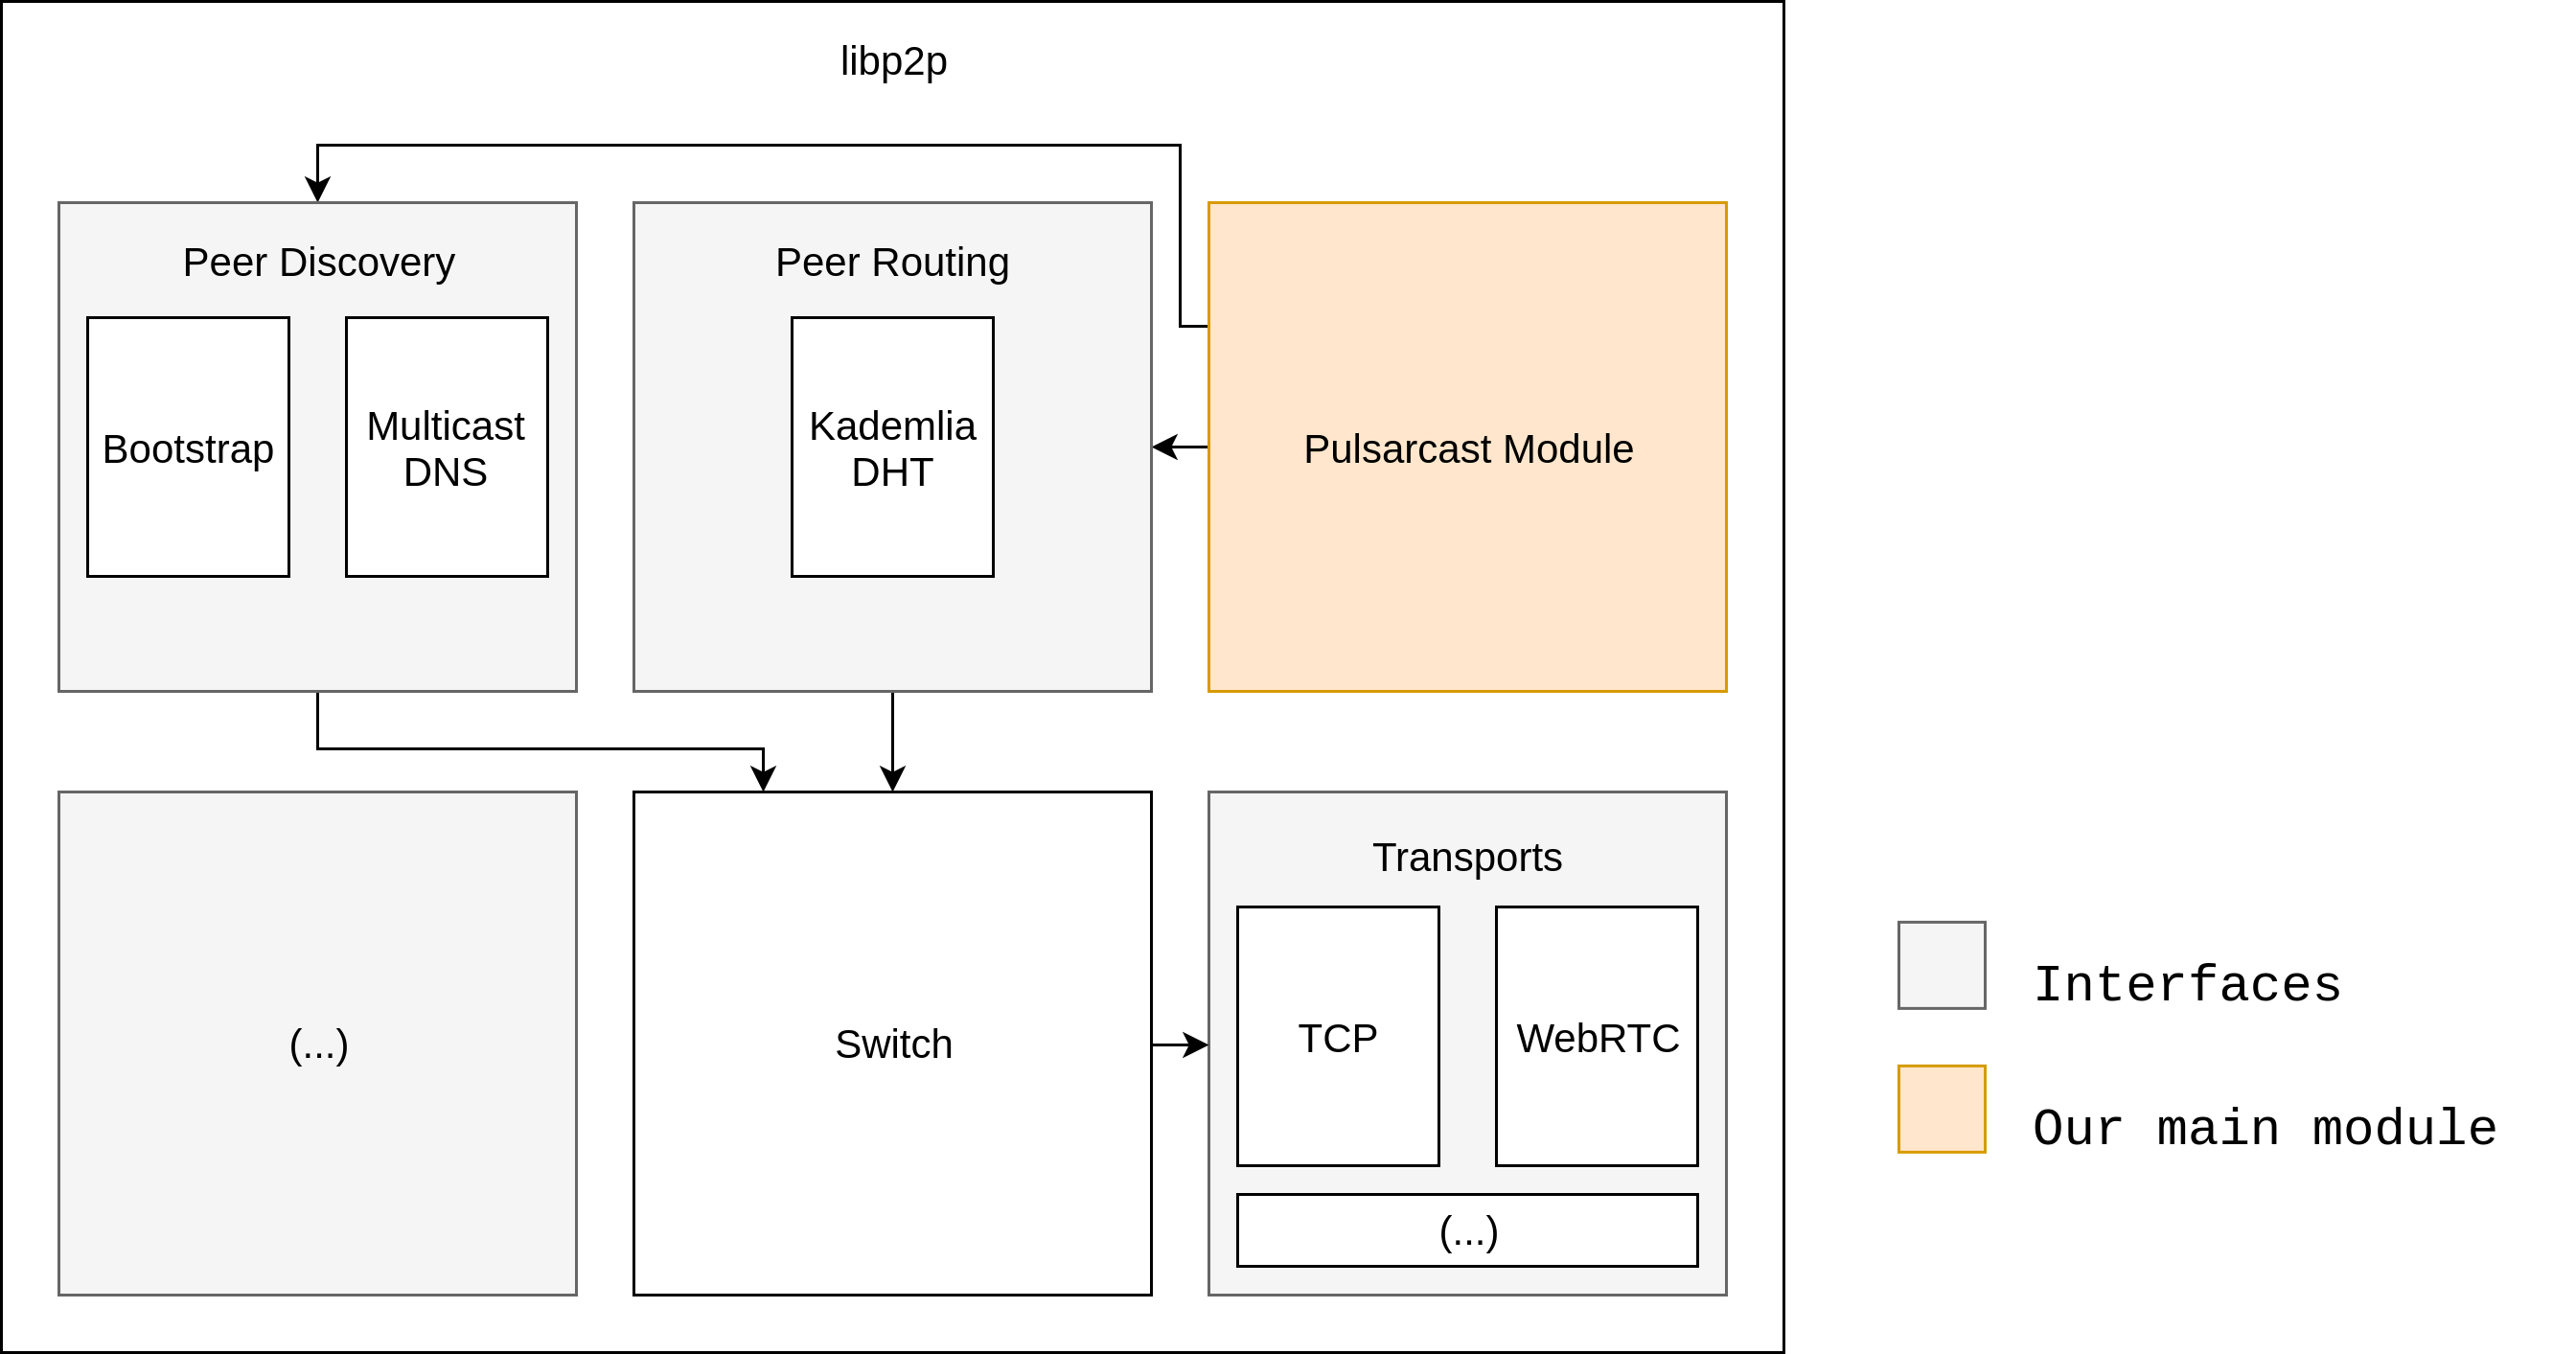
\includegraphics[width=0.95\textwidth]{img/pulsarcast-in-libp2p.png}
  \caption{Our Pulsarcast module in the libp2p ecosystem}
  \label{fig:pulsarcast-in-libp2p}
\end{figure}

\begin{figure}[hb!]
  \center
  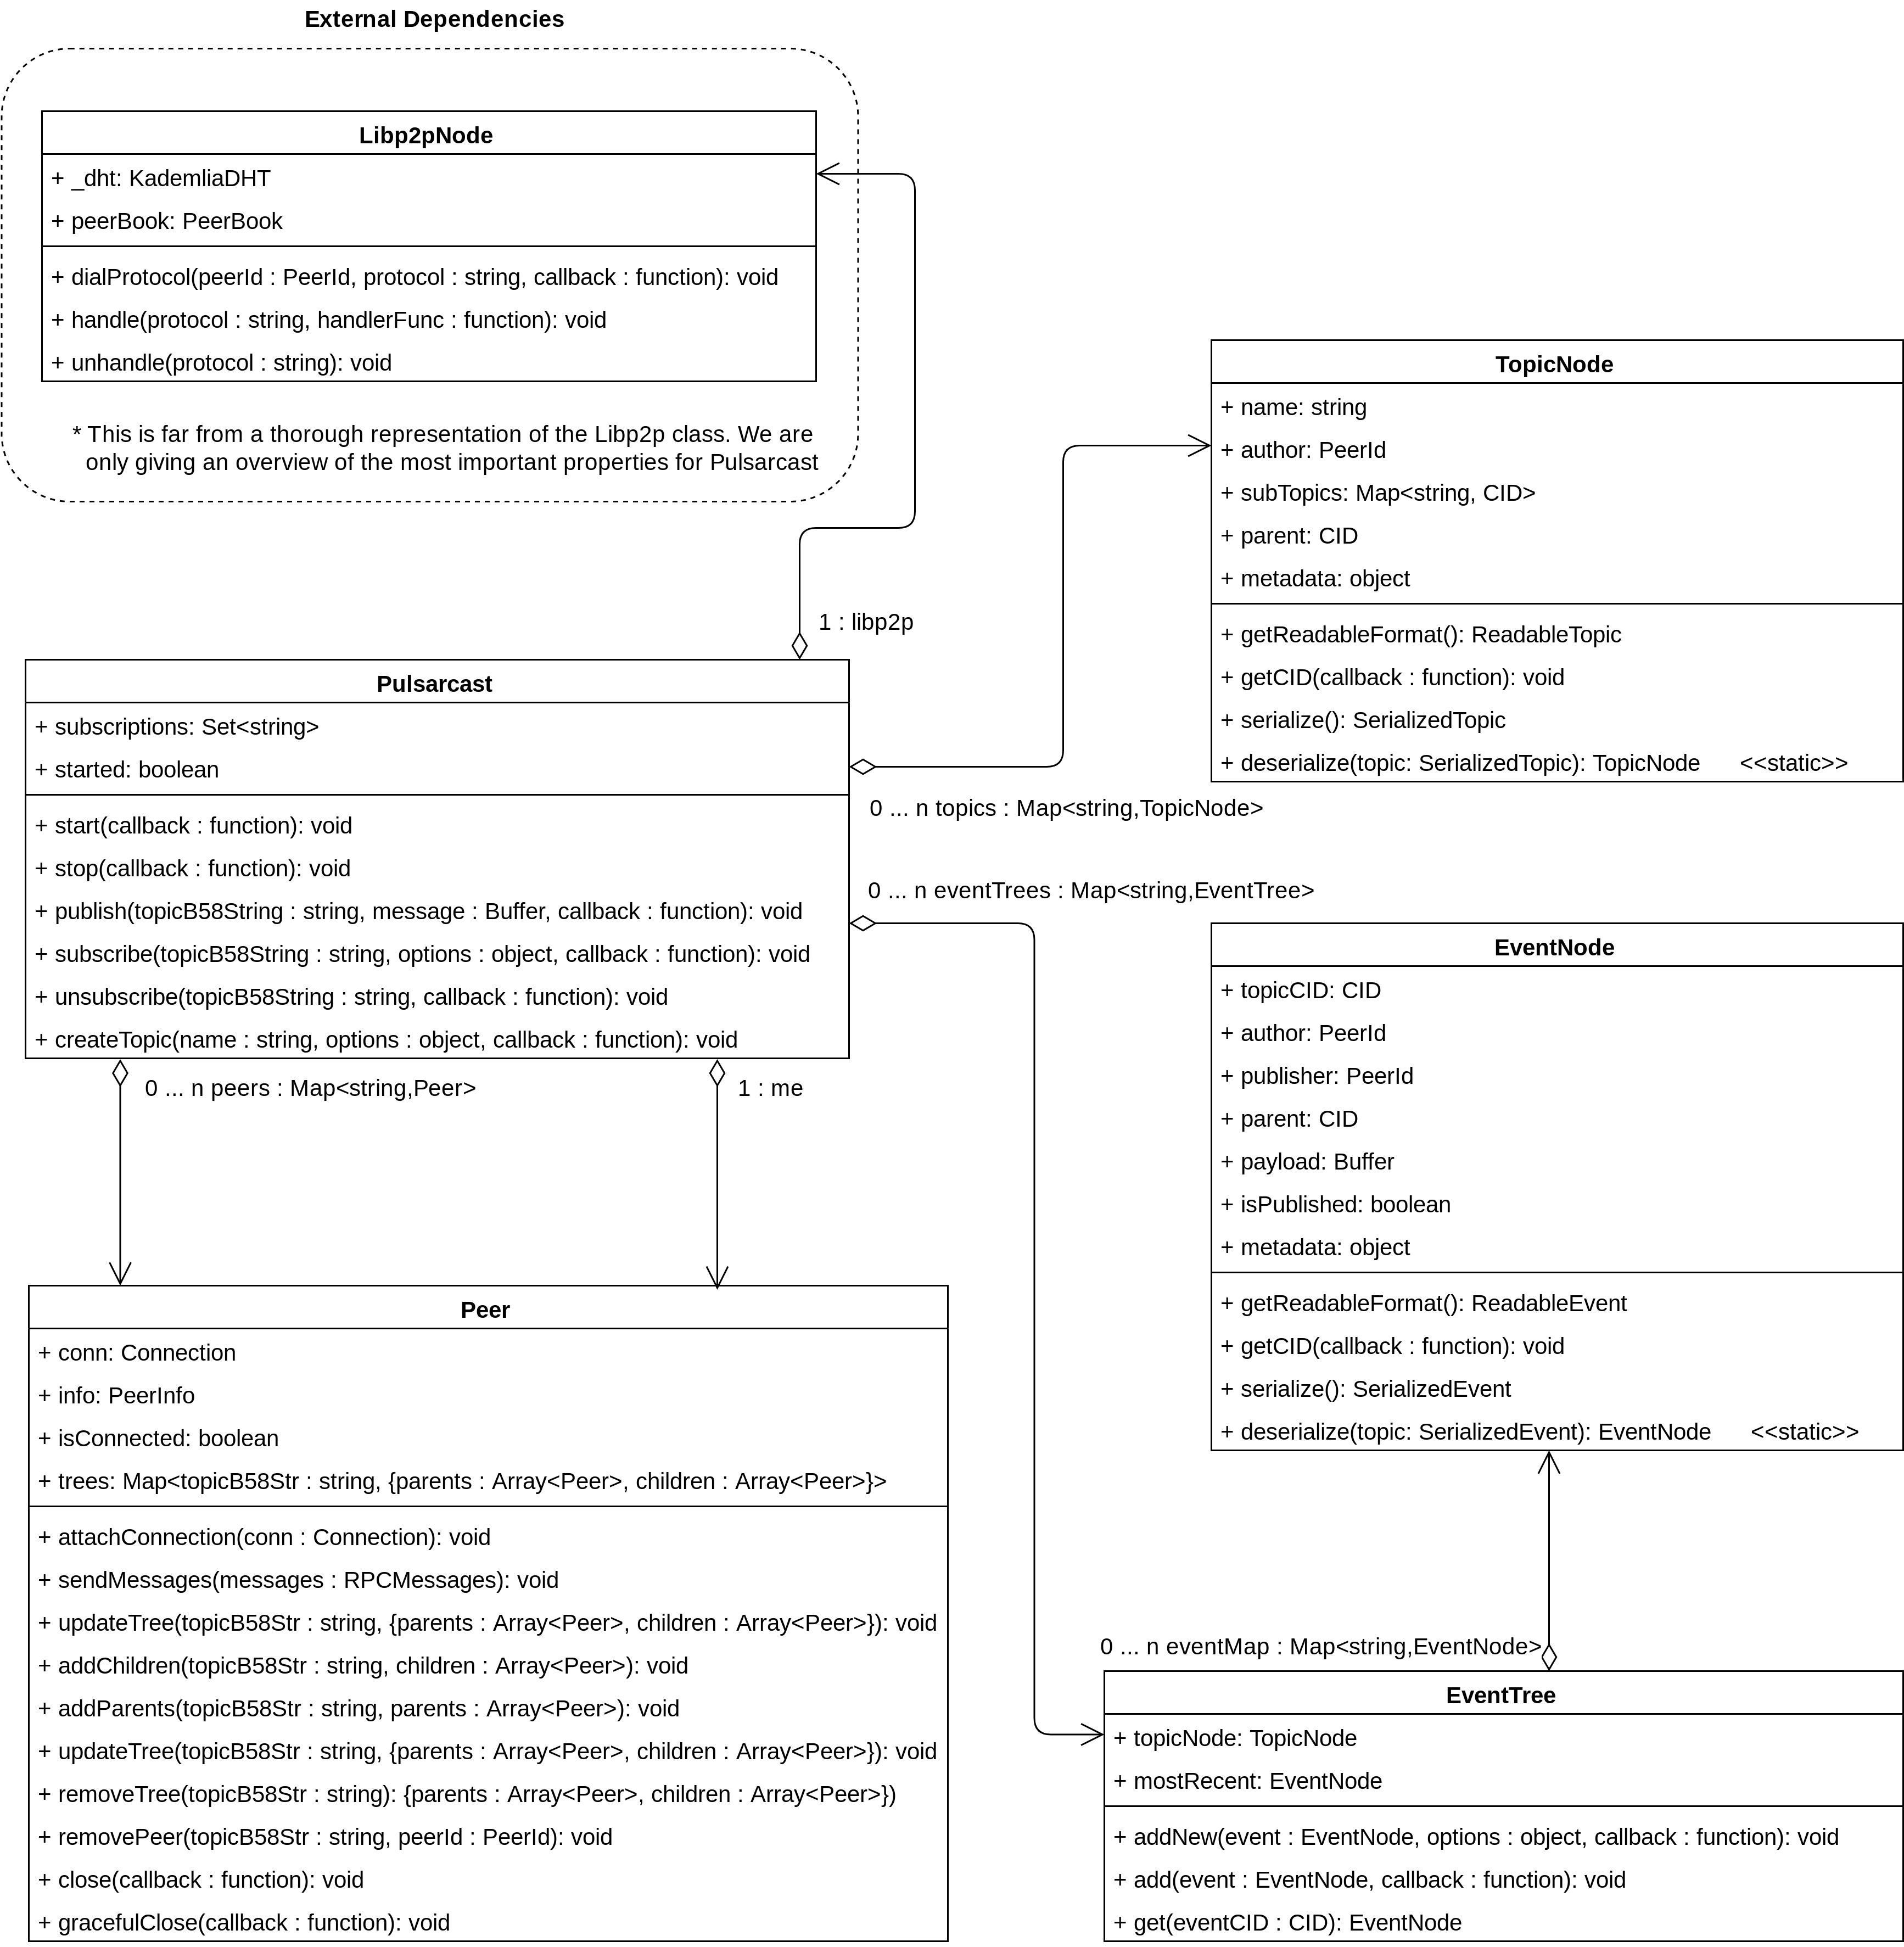
\includegraphics[width=1\textwidth]{img/uml-pulsarcast.png}
  \caption{UML representation of the classes in our Pulsarcast system}
  \label{fig:pulsarcast-uml}
\end{figure}

\section{Testbed}\label{testbed}

TODO

\section{Summary}\label{summary}

TODO
